
\documentclass{standalone}

\usepackage{graphics}
\usepackage{tikz}
\usetikzlibrary{positioning}
\usetikzlibrary{arrows.meta}

\begin{document}
\scalebox{1.5}{
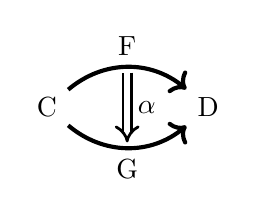
\begin{tikzpicture}[line width=1.5pt]

	\node (C) {C};
	\node (D) [right=1.5cm of C] {D};

	\draw[->, bend left=40] (C) to coordinate (m1)  (D) ;
	\draw[->, bend right=40] (C) to coordinate (m2)  (D);

	\draw[
		-Implies,line width=1.pt,double distance=2pt,
		shorten <=2pt, shorten >=2pt,
	] (m1) -- node [right] {$\alpha$} (m2) ;

	\node [above] at (m1) {F};
	\node [below] at (m2) {G};

\end{tikzpicture}
}

\end{document}

